\documentclass[a4paper,11pt]{report}
%FONT size can be changed on the above line
\usepackage[left=2.7cm,right=2.7cm,top=4cm,bottom=3.5cm,bindingoffset=0cm]{geometry}
%%% Headers
\usepackage{fancyhdr}
\renewcommand{\chaptermark}[1]{%
\markboth{#1}{}}  
\pagestyle{fancy}
\fancyhead[LO]{}
\fancyhead[RE]{}
\fancyhead[LE]{\textit{\leftmark}}
\setlength{\headheight}{15pt}

%%%%
\usepackage{tabularx}
\usepackage{amsmath}
\usepackage{amssymb}
\usepackage{ntheorem}
\usepackage{graphicx}
\usepackage{setspace}
\usepackage[outdir=./]{epstopdf}
\usepackage{caption}
\usepackage{subcaption}
\usepackage{array}
\usepackage{paralist} 
\usepackage{datetime}
\usepackage{verbatim}
\usepackage{makeidx}
\usepackage{titling}
\usepackage{titlepic}
\usepackage{enumitem}
\usepackage[toc,page]{appendix}
\usepackage[breaklinks=true]{hyperref}
\usepackage{pdfpages}
\usepackage{mathrsfs}
\usepackage{etaremune}
 \usepackage{bm}
\usepackage{sansmath}
\usepackage{pgfplots}
\usepackage{mdframed}
\usepackage{tikz}
\usepackage{tikz-3dplot}
\usepackage{stmaryrd}
%%Fix line breaks for long citations
\usepackage{breakcites}
\usepackage{siunitx}
\usepackage{tocbibind}
\usepackage{lipsum}
\renewcommand{\epsilon}{\varepsilon}
\usepackage{biblatex}
\addbibresource{references.bib}

\mdfdefinestyle{MyFrame}{%
%    linecolor=blue,
        linewidth=1pt,
%    roundcorner=20pt,
%    innertopmargin=\baselineskip,
%    innerbottommargin=\baselineskip,
%   innerrightmargin=20pt,
%    innerleftmargin=20pt,
%    backgroundcolor=gray!50!white
}
\usepackage{svg}
\usepackage{listings}
%New colors defined below
\definecolor{codegreen}{rgb}{0,0.4,0}
\definecolor{codegray}{rgb}{0.5,0.5,0.5}
\definecolor{codepurple}{rgb}{0.58,0,0.82}
\definecolor{backcolour}{rgb}{0.95,0.95,0.92}

\lstdefinestyle{mystyle}{
  backgroundcolor=\color{backcolour}, commentstyle=\color{codegreen},
  keywordstyle=\color{magenta},
  numberstyle=\tiny\color{codegray},
  stringstyle=\color{codepurple},
  basicstyle=\ttfamily\small,
  breakatwhitespace=false,         
  breaklines=true,                 
  captionpos=b,                    
  keepspaces=true,                 
  numbers=left,                    
  numbersep=5pt,                  
  showspaces=false,                
  showstringspaces=false,
  showtabs=false,                  
  tabsize=4
}
\lstset{style=mystyle,upquote=true}

\begin{document}


\begin{titlepage}
    \begin{center}

    \vspace{30pt}
    
\includegraphics[width=0.5\textwidth]{figures/ATULogo.png}\\
    \vspace{50pt}
    
    \fontsize{14}{20} \selectfont
    
    \textbf{\Huge COVID - 19 Automated Detection using Convolutional Neural Networks and Generative Adversarial Networks} 
    \vspace{40pt}
    
    A thesis submitted \\
    by\\
    \vspace{15pt}
    
    {\huge Ultan Kearns}\\
    \vspace{15pt}
    
     in partial fulfillment of the requirements for the degree of\\ Master of Science in Computing in Big Data Analytics and Artificial Intelligence
    \vspace{40pt}

%        \fontsize{16}{20} \selectfont
    
    
    Supervisor: Dr Paul Greaney
    \vspace{100pt}
    
    
Submitted to Quality and Qualifications Ireland (QQI) \\
Dearbhú Cáilíochta agus Cáilíochtaí Éireann
    \centerline{\monthname \quad \the\year}
\end{center}    
\end{titlepage}

\onehalfspace


\setcounter{page}{1}

%\setcounter{tocdepth}{2}

\addtocontents{toc}{\protect\setcounter{tocdepth}{-1}}
\tableofcontents
\addtocontents{toc}{\protect\setcounter{tocdepth}{2}}

%\listoffigures

\chapter*{Declaration}
\addcontentsline{toc}{chapter}{Declaration}

I hereby certify that this material, which l now submit for assessment on the programme of study leading to the award of Master of Science in Computing in \dots, is entirely my own work and has not been taken from the work of others except and to the extent that such work has been cited and acknowledged within the text of my own work. No portion of the work contained in this thesis has been submitted in support of an application for another degree or qualification to this or any other institution. I understand that it is my responsibility to ensure that I have adhered to LYIT’s rules and regulations. 
\bigskip

I hereby certify that the material on which I have relied on for the purpose of my assessment is not deemed as personal data under the GDPR Regulations. Personal data is any data from living people that can be identified. Any personal data used for the purpose of my assessment has been psudonymised and the data set and identifiers are not held by LYIT. Alternatively, personal data has been anonymised in line with the Data Protection Commissioners Guidelines on Anonymisation.
\bigskip

I give consent for my work to be held for the purposes of education assistance to future Computing students at LYIT and it will not be shared outside the Department of Computing at LYIT. I understand that my assessment may be shared with any other third party and will be held securely in LYIT in line with the Institute's Records Retention Policy. 

\vspace{20pt}

\hspace{60pt} Signed: \underline{\quad \quad Ultan Kearns\hspace{240pt}} 


\bigskip

\hspace{70pt} Date: \underline{\quad \quad\today\hspace{150pt}} 

\begin{abstract}
    This paper aims to analyze the applications of generative adversarial networks or GANs in overcoming issues of data-shortages in relation to developing convolutional neural networks to automate the diagnosis of COVID-19 in patients.  There have been many COVID-19 data-sets compiled but some suffer from lack of data-quality and data shortages\cite{covid19DataQuality}\cite{covid19DataQuality2}.  In this paper I aim to create and train multiple convolutional neural networks or CNNs to analyze X-Rays of patients lungs to automate the detection of COVID-19.  The CNN will be trained with a number of images generated from different GAN architectures to determine which will prove most efficient in automating the detection of COVID-19.  I also aim to use the GANs in conjunction with one and other to try out different combinations to see if feeding images generated by one GAN to other GANs will produce more accurate results when training the model.  In the results section of this Thesis I will compare and contrast the results of the various architectures and determine which proved most effective in it's diagnostic potential.
\end{abstract}

\chapter{Introduction}

\section{Explanation of Generative Adversarial Networks (GANs)}
A generative adversarial network or GAN for short first appeared in a 2014 paper by Ian Goodfellow et al\cite{generativeAdversarialNetworks}.  In this paper Goodfellow et al propose a new way to generate data via an adversarial process.  The GAN essentially works as follows: two models are trained, a generative model $G$ which will generate the synthetic data from the real data and another model $D$ which will be the discriminator, judging if the data was created by the model or if it came from the dataset.  The goal of this training is to ensure data generated from $G$ is realistic enough to make the discriminator $D$ believe that the generated content came from the training set, this is achieved by training the model for a number of epochs and adjusting the models weights to improve the quality of the generated image.  It  is in this way that we can create realistic "fake" data from the generative model.
\\
There are a number of GAN architectures which are useful in different scenarios, such as CycleGans\cite{cycleGan} which are useful for translating images from a source domain $X \rightarrow Y$ in which $Y$ is the target domain, StyleGan, which was created by NVIDIA which allows more control over the generative process\cite{styleGan} and PixelRNN, which can recreate images when given a fraction of the original and can generate new images based on probability\cite{pixelRnn}. 
\\
This dissertation examines a number of different generative adversarial network architectures and their ability to produce meaningful data when trained on the datasets which will be mentioned in a later section.
\vspace{0.5mm}
\begin{figure}[H]
    \centering
    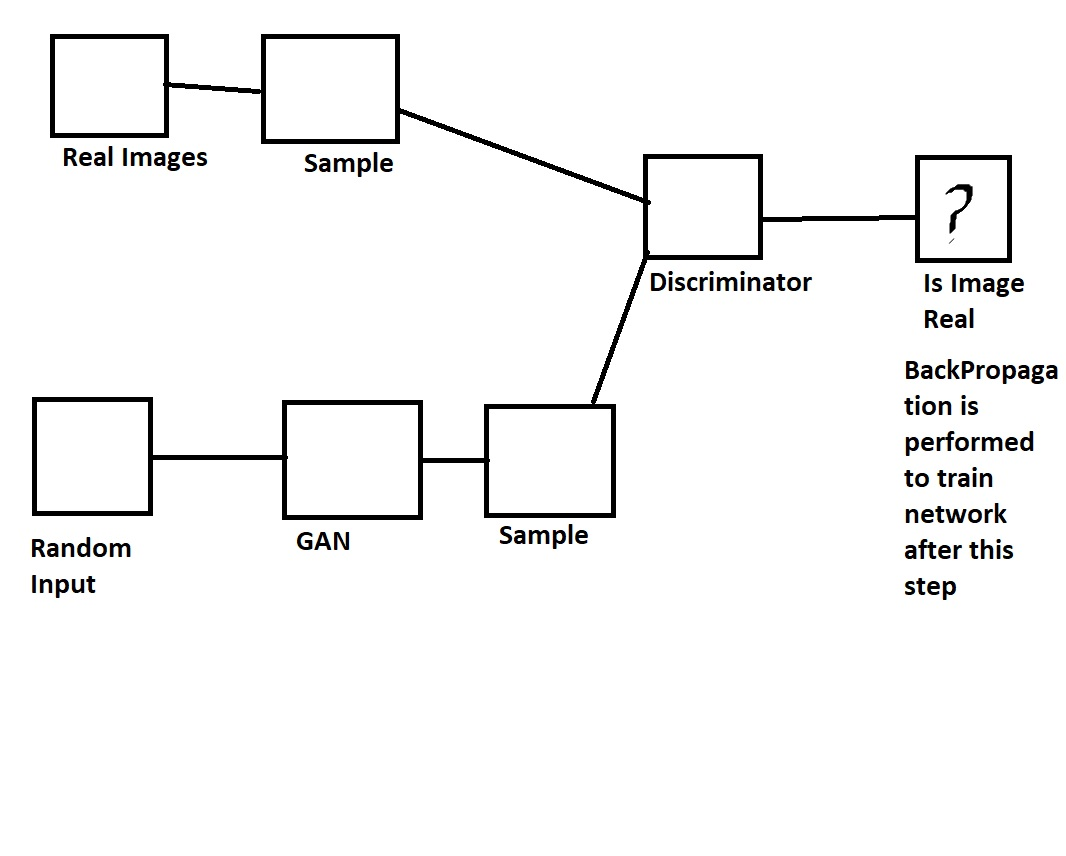
\includegraphics[width=1\textwidth,height=10cm]{Images/GAN Basic.jpg}\\
    \caption{Basic Example of Generative Adversarial Network}
    \label{fig:Example GAN Diagram}
\end{figure}
\vspace{0.5mm}
As we can see from the image above \ref{fig:Example GAN Diagram}, we start the process by taking a sample of real images from the training data, then passing it to the discriminator. We also take a sample from the GAN created images and pass that to the discriminator which will then determine if the images are real are fake.  After the discriminator guesses if the image generated is good enough to be considered real in terms of quality then backpropagation is performed to train the model so that it can differentiate better between samples that came from the training set and those which came from the generator $G$.
\section{Explanation of Artificial Neural Networks (ANNs)}
Artificial Neural Networks, or ANNs for short, comprise of a network of neurons or nodes(both terms can be used interchangeably) which are used for training a model to perform a certain task.  They are made up of an input layer, $N$ hidden layers, and finally an output layer.  Each layer has its own activation function and will adjust its weights and biases to determine the final output of the model.\cite{introToCnn} These networks are  heavily inspired by biological processes which occur in the brain.
\\
Artificial neural networks are a general-purpose model used to solve a number of common problems.
\vspace{0.5mm}
\begin{figure}[H]
    \centering
    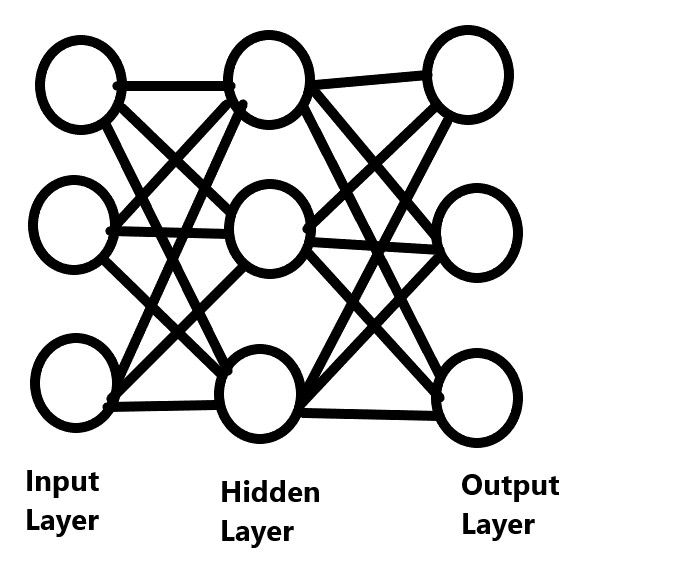
\includegraphics[width=0.5\textwidth]{Images/ANN Basic.jpg}\\
    \caption{Diagram of a Basic Artificial Neural Network with 1 input layer, 1 output layer, and 1 hidden layer}
    \label{fig:Example ANN Diagram}
\end{figure}
\vspace{0.5mm}

A basic example of an artificial neural network is shown in Figure \ref{fig:Example ANN Diagram}. As shown in the figure, the network has an input layer, a hidden layer, and an output layer.  Generally when creating these networks we determine the number of neurons in both the input and the output layers based on the number of classes we are trying to predict.  The above network could be used to predict if an image is of a cat, a dog, or a fish for example.  There can multiple hidden layers in an ANN and the number of neurons in each layer can be adjusted.  In reality, artificial neural networks will typically be far bigger than the example given above in terms of neurons and hidden layers but for illustrative purposes, the above diagram will suffice.  Each neuron will also have its own weight, bias, and an activation function which will determine whether a neuron fires or not. There are many common activation functions such as swish, ReLU (Rectified Linear Units), sigmoid, and tanh the use of which depends on a number of factors.
\section{What is A Convolutional Neural Network? (CNN)}
A convolutional neural network, or CNN for short, is a type of neural network which is primarily used for tasks involving image and pattern recognition\cite{introToCnn}. The structure is similar to an ANN in which we have an input layer, $N$ hidden layers, and finally an output layer.  As with the Artificial Neural Network each of these layers will have an activation function and its own weights and biases to determine the final output for a given input. The model will take an image as input, the image is made up of vectors (RGB) or a similar format and from that image the model will determine certain patterns. For example, the output might be a classification of whether or not COVID-19 is present. This application will be discussed in more detail later in the dissertation. 
\\
There are a few ways in which CNNs differ from ANNs, in that they are comprised of three types of layers which are the convolutional layers, pooling layers, and fully connected layers\cite{introToCnn}.  The convolutional layer is responsible for extracting features from an image and generating a $2D$ activation map, the pooling layer will reduce the parameters of a given input by means of downsampling, and finally the fully connected layers will then determine and classify the output for a given input.  The convolutional layer's parameters utilize learnable kernels (a kernel acts as a filter used to extract features from images), and this layer also produces a $2D$ activation map which will be used to determine if a neuron fires or not for a given input.  We can adjust hyper parameters in the convolutional layer to greatly reduce the complexity of the model through optimization, which can be achieved by adjusting the following hyper parameters: depth, stride and zero padding.
\\
Depth is related to the output volume produced by the convolutional layers in the model which can be manually set by adjusting the number of neurons in each layer.  Reducing the depth of the model can greatly decrease the training time but at the expense of performance.
\\
Stride is related to the spatial dimensionality of the input which will determine the receptive field (this is an area where each neuron in the network is connected to a small region of the input - this area of the network is called the receptive field\cite{introToCnn}), if the stride is set to a low integer we will produce extremely large activations, and if it is set too high the network won't produce enough activations.  The stride can also be interpreted as sliding a window across the image / video, where only a section of the image or video is input into the network at a time.
\\
Finally, zero-padding will pad the border of the images ingested by the model with 0s, reducing their dimensionality. Padding can prove to be useful in increasing the accuracy of the model as it can possibly eliminate areas of the image which are not useful for the model and can also improve training time times in some use cases\cite{zeroPaddingTrainingTime}.
\\
Through the adjustment of the hyperparameters mentioned above, and through the utilization of different activation functions, the accuracy of the convolutional neural network can be improved through a process of trial and error.
\section{Supervised Learning}
Supervised learning is a methodology of machine-learning involving the use of labeled data to train the model\cite{supervisedVsUnsupervised}. The data is typically labeled manually by a data scientist, which can be a long and laborious process depending on a number of factors (size of the data, number of classes, etc.), but offers many benefits when it comes to training models.  Supervised learning performs extremely well at tasks involving classification (classifying data into a given category), and regression (understanding the relationships between independent and dependent variables). 
\section{Unsupervised Learning}
Unsupervised learning is a methodology of machine-learning which involves using unlabelled data to train machine learning models\cite{supervisedVsUnsupervised}.  This type of machine learning requires no human intervention since the data is unlabelled and the model will detect relationships between data based on the raw data fed in to the model.  This type of machine learning is used for tasks such as: clustering (grouping data together based on shared characteristics or features), association (finding relationships between features), and dimensionality reduction (reducing the number of features in a given dataset without compromising the integrity of said data).  The key differences between supervised and unsupervised learning are: labeled versus unlabeled datasets, and finding relationships in data (unsupervised) or trying to predict and classify data (supervised).
\section{Tensorflow}
Tensorflow is an open-source library which allows developers to access a number of functions to make machine learning easier and allows developers to build models more quickly\cite{tensorflow}.  Tensorflow provides numerous modules and classes which form the foundation for building both the generative adversarial network and the convolutional neural network. There have been numerous case studies proving the efficacy of Tensorflow in solving many AI / ML problems and the library is used by research teams in organisations such as Google, Airbnb, ARM, Coca-Cola, Intel, and many more\cite{tensorflowCaseStudies}.  
\\
Given the reputation and widespread use of Tensorflow, and the vast amount of documentation around the framework, it seems  an ideal library for the implementation of GANs and CNNs for this study.
\section{Keras}
Keras is a deep-learning framework for Python developed by Francois Chollet which provides a number of helpful functions and methods for creating AI models\cite{keras}. Keras is built on top of Tensorflow and simplifies data loading, pre-processing and the overall building of the model.  Keras is commonly used by data-scientists and researchers due to the powerful methods it offers and the time it saves.  The additional classes and modules Keras provides on top of Tensorflow will help to reduce the time taken to build and develop of building both the convolutional neural network and the generative adversarial network.  
\\
Like Tensorflow, Keras has been used by a number of companies and is well recognised in the Artificial Intelligence community.  The framework has a range of uses and has proven beneficial when developing AI models in a number of areas and fields\cite{kerasExamples}.
\section{Background of Problem \& Aims of This Paper}
COVID-19 is a highly transmissible virus which has caused a worldwide pandemic and has claimed many lives. There have been 616,951,418 cases worldwide and 6,530,281 deaths as of the 4th of October 2022\cite{covid19StatsWorldwide}.  During the pandemic, Ireland alone was subject to a total of 1.6 million confirmed cases and nearly 8,000 deaths\cite{covid19StatsIreland}.  This has led many researchers to pursue the goal of automating the detection of COVID-19 to partially relieve the immense pressure put on medical staff throughout the pandemic. 
\vspace{0.5mm}
\begin{figure}[H]
    \centering
    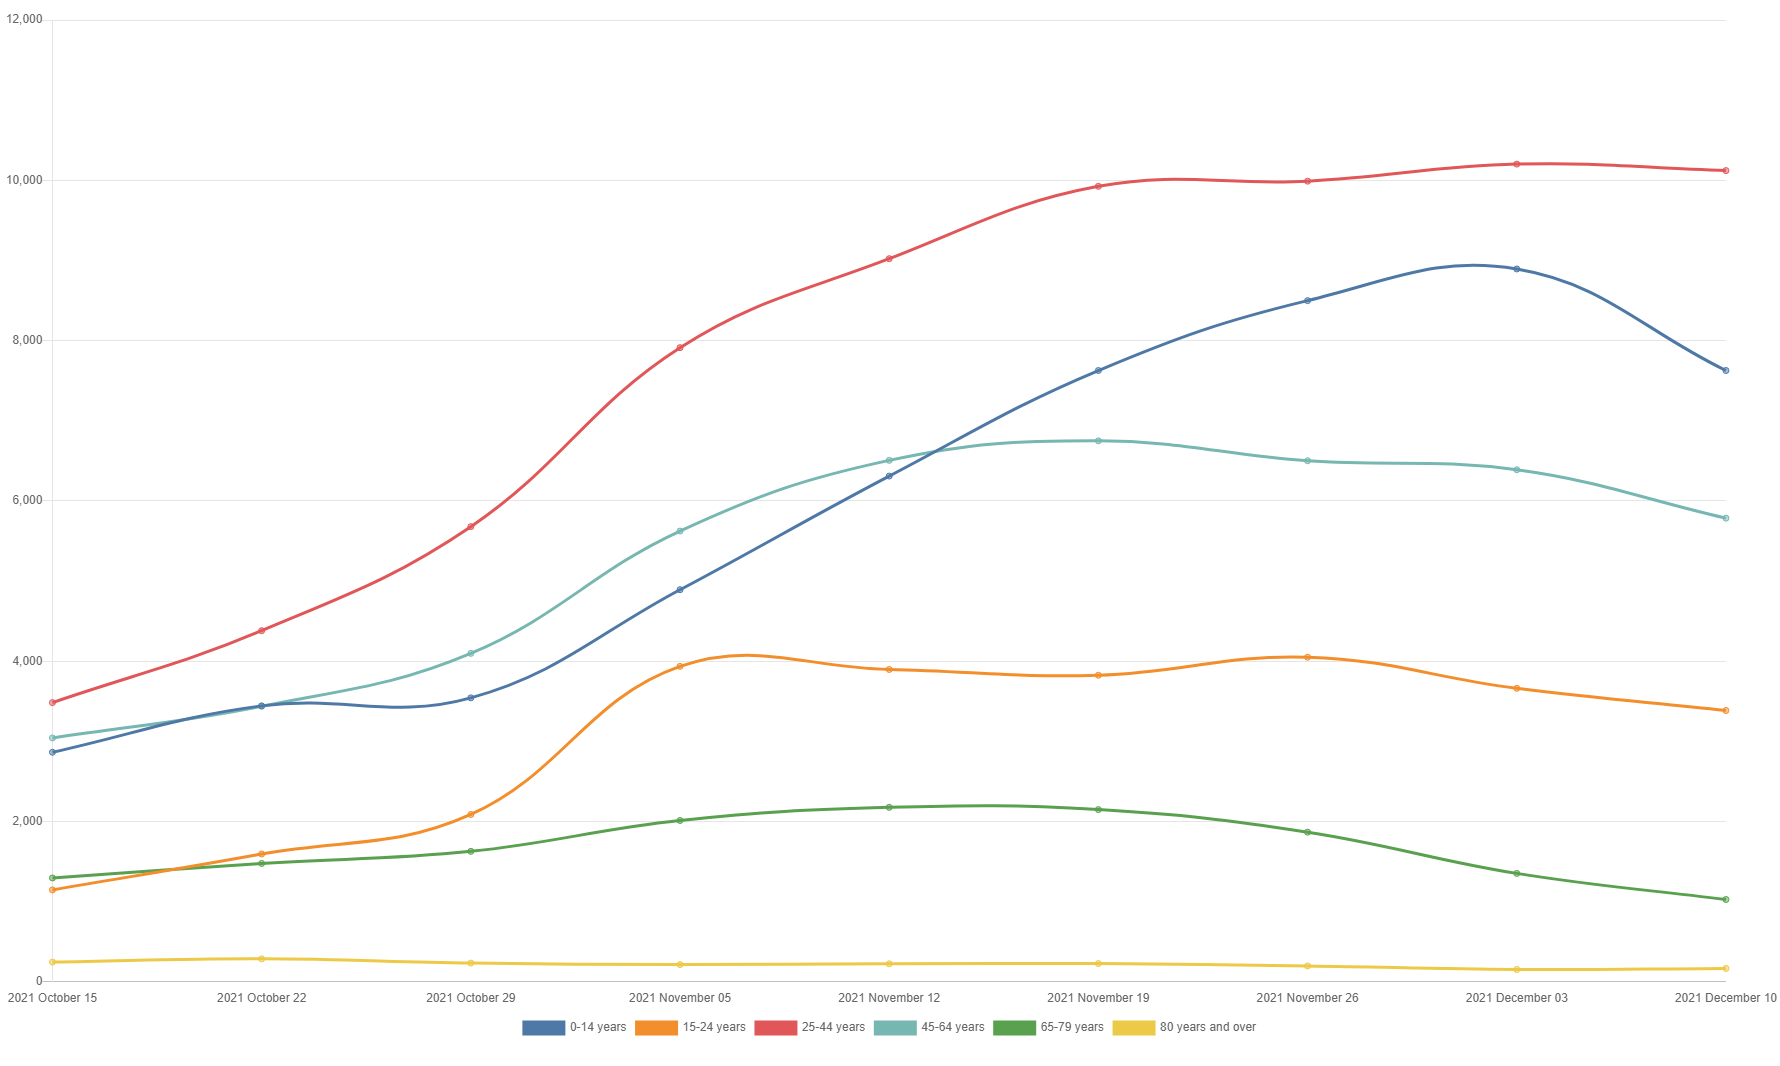
\includegraphics[width=1\textwidth,keepaspectratio]{Images/COVID19IrelandFigures.png}\\
    \caption{Graph of COVID-19 Statistics by age-range Ireland from October 2021 - December 2021 Courtesy of CSO\cite{csoCovid19Stats}}
    \label{fig:COVID-19 Ireland Statistics}
\end{figure}
\begin{figure}[H]
    \centering
    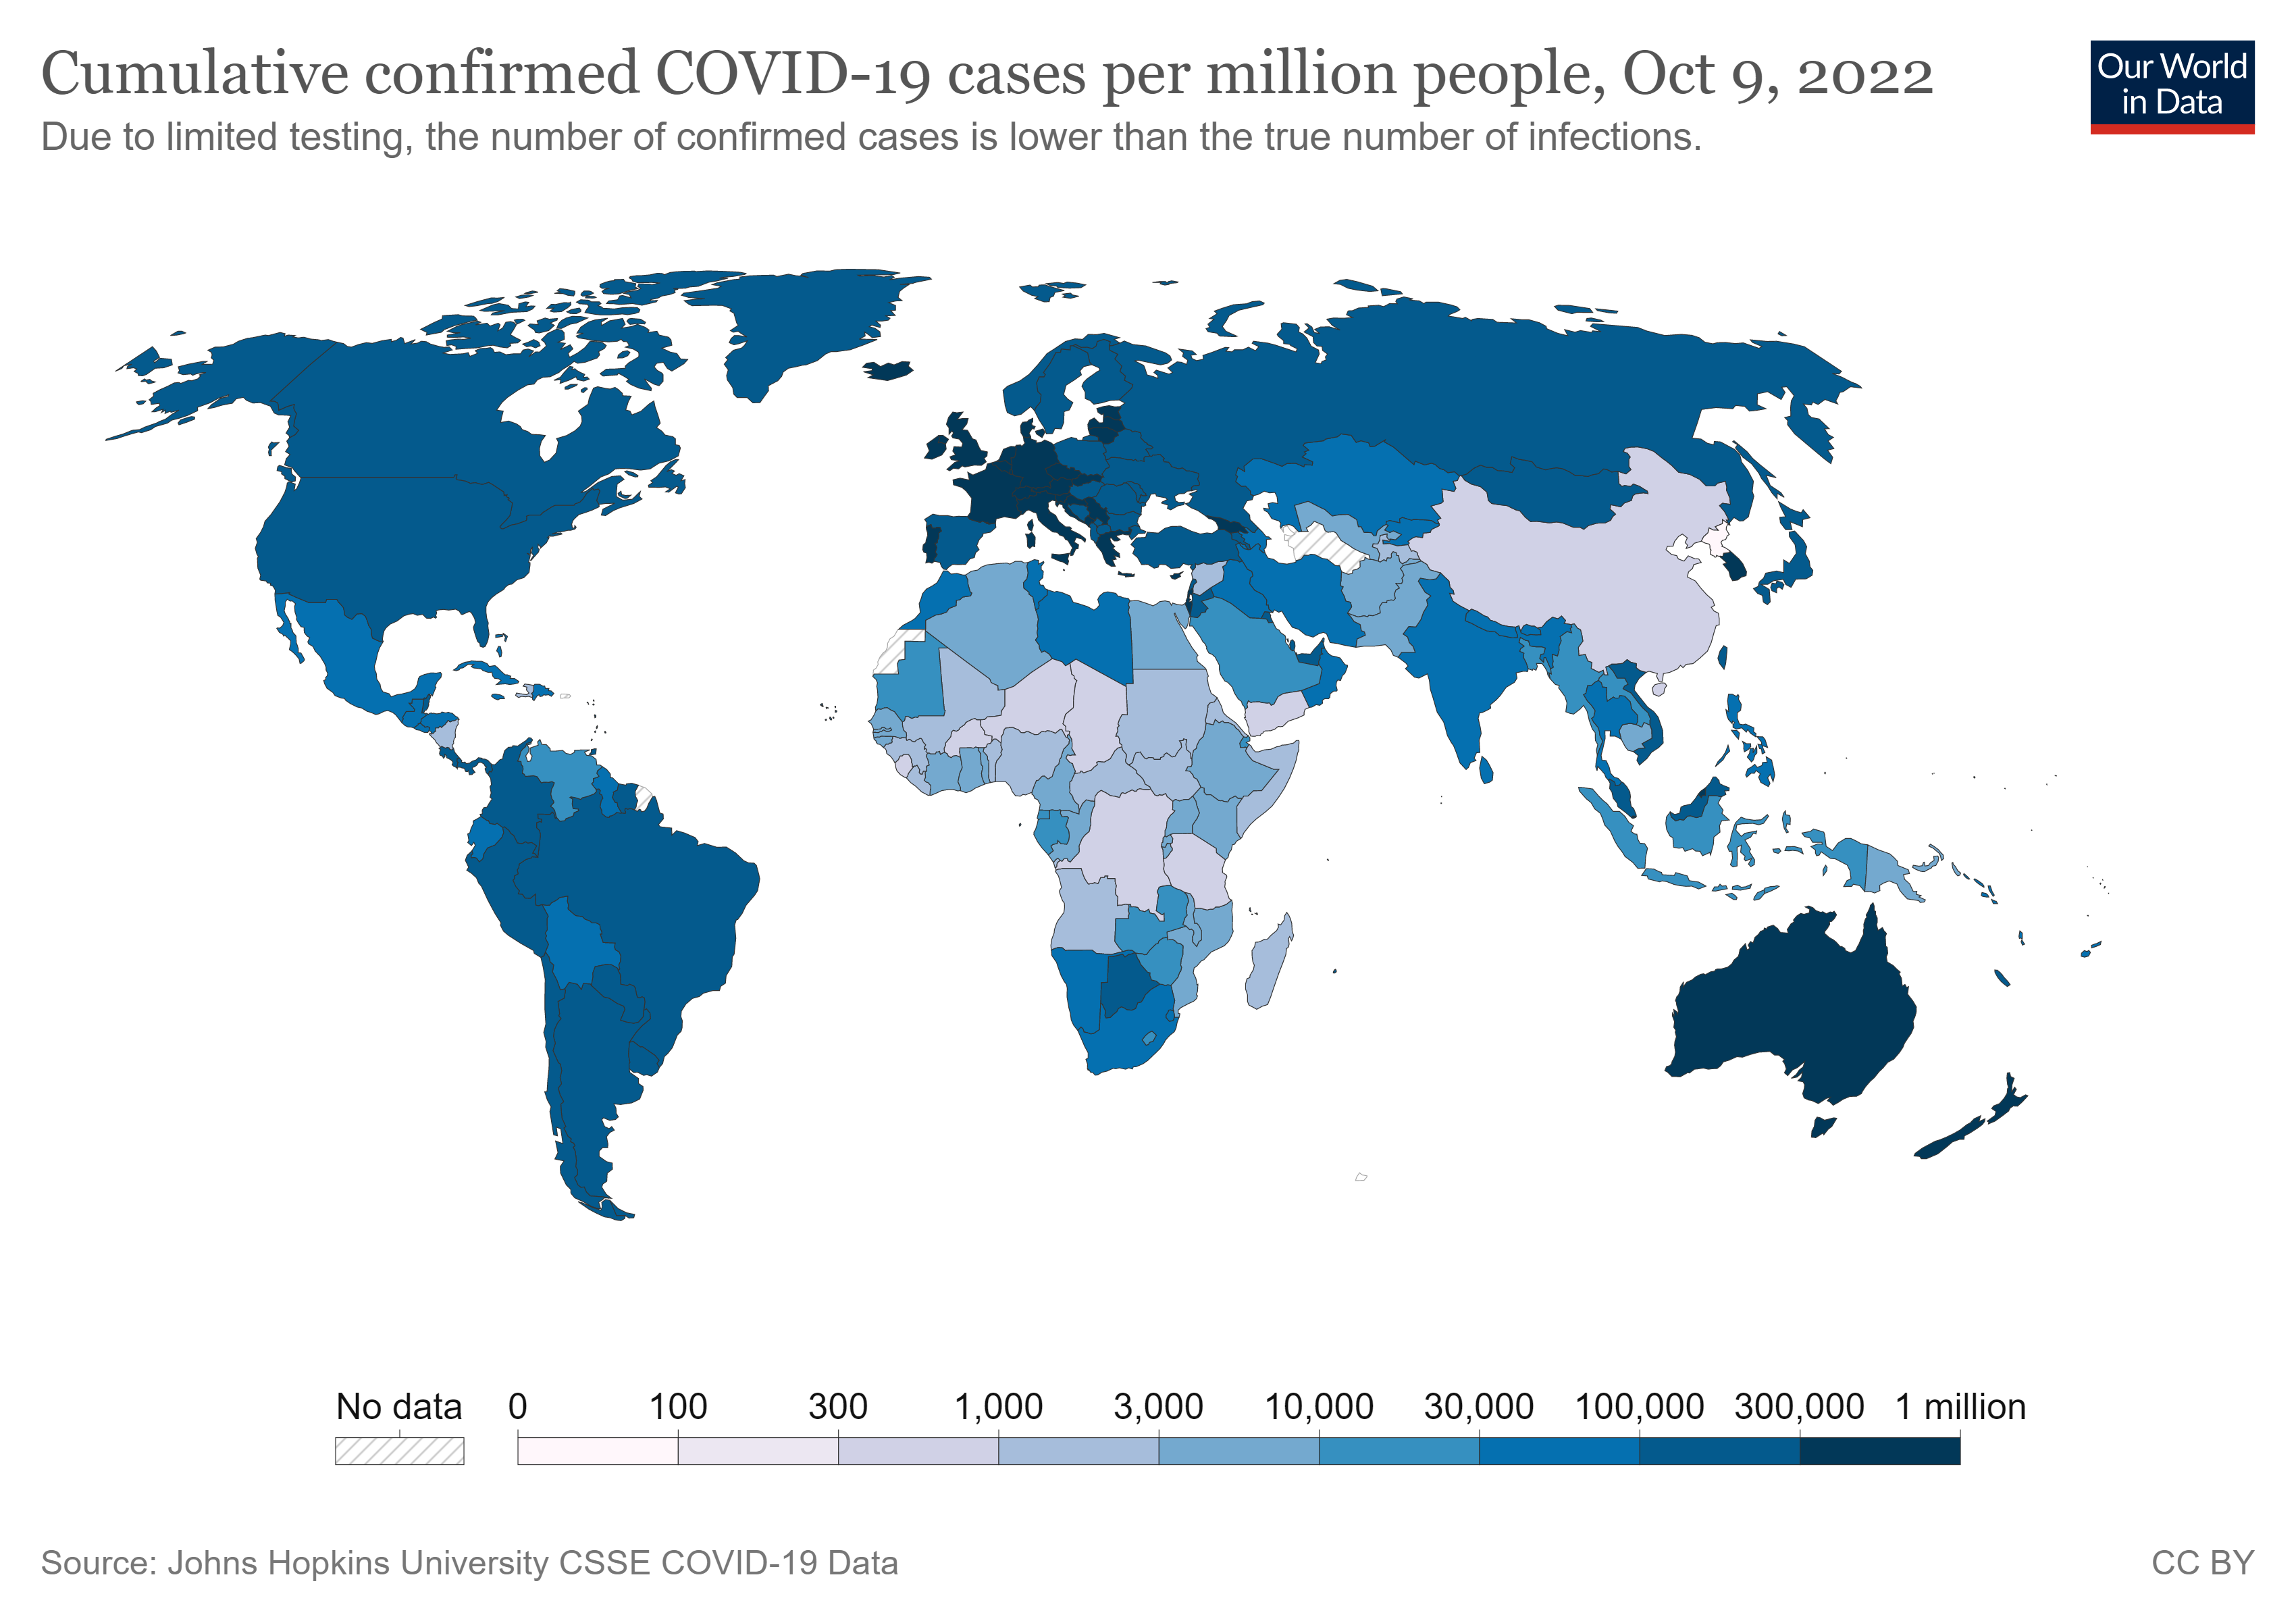
\includegraphics[width=1\textwidth,keepaspectratio]{Images/coronavirusWorldWide.png}\\
    \caption{Cumulative cases of the COVID-19 virus worldwide courtesy of Our World in Data\cite{cumulativeCovid19Cases}}
    \label{fig:COVID-19 Worldwide Statistics}
\end{figure}
\vspace{0.5mm}
The main objective of this research is to develop a robust model which can accurately analyze X-rays of patients and determine from said X-rays if the patient is afflicted with COVID-19.  This will be achieved by utilizing a number of different GAN architectures which will create realistic ''fake data'' which will then be used to train a number of models. From this training we plan to compare and contrast the results when generating data with different architectures to determine the best configuration for data generation to train the CNN model.  There has been some success in utilizing convolutional neural networks to automate the detection of the virus\cite{cnnCOVID19DetectionAhmed}\cite{cnnCOVID19DetectionLopez}.  Through the use of synthetic data generated by utilizing a variety of GAN architectures, it is our hope that such convolutional models will be improved upon and made more accurate.
\\
We plan on utilizing existing data sets which are listed in the next section when training the Generative Adversarial Models, through trial and error we plan on determining the best architecture of GANs to use for training the model for this use-case.
% Include stats and explain COVID 19 virus
\section{Datasets}
Before beginning the training of the model it is important to explore and understand each of the datasets.  There are a total of three datasets which will be used in the course of this research, we will explain more about these datasets below.
\subsection{COVID-19 Chest X-ray}
The COVID-19 Chest X-ray data set is a data set which is comprised of labeled X-ray Images taken from a number of patients. This dataset contains 357 X-ray images of COVID positive patients, and Chest X-rays of those afflicted with another disease (MERS, SARS, and ARDS).  This dataset also includes a metadata file listing the diagnosis of the patient along with a number of other features\cite{xrayDataset}. In total this dataset contains 11 classes, the images do not have a consistent resolution which may cause issues as resizing each image may lead to a loss in image quality.  The loss in quality will cause problems when evaluating the model's accuracy.
\\
\subsection{COVID-19 Radiography Database}
The COVID-19 Radiography Database is made up of 3,616 images of chest X-rays taken from COVID positive patients, 10,192 Images of lung X-rays taken from healthy patients, and 1,345 X-ray images of viral pneumonia positive patients. All images in this dataset are PNG (Portable Network Graphic) images and are at a resolution of height 299 pixels and width 299 pixels eliminating the need for preprocessing of the images, the dataset also includes metadata for each of the images in this dataset showing a number of features with the diagnosis of the patient as well. The data in this dataset was gathered by a team of researchers from Qatar University, Doha, Qatar, and the University of Dhaka, Bangladesh along with their collaborators from Pakistan and Malaysia\cite{radiography}.
\\
\subsection{COVID-19 Pneumonia Normal Chest X-ray PA Dataset}
The COVID-19 Pneumonia Normal Chest X-ray PA dataset is comprised of a train set containing 74 Normal X-ray Images taken from healthy Patients and  afflicted with Pneumonia and a test set containing a Normal set containing 20 chest X-rays taken from healthy patients and a Pneumonia set containing 20 images.  The images in this dataset are unlabelled and no metadata is offered, however, the images are segregated into separate files listing the diagnosis\cite{covidDataset}.
\\
\subsection{Extensive COVID-19 X-ray and CT Chest Images Dataset}
This dataset was added fairly late in the project due to data limitations in both the COVID-19 Chest X-ray and the COVID-19 Pneumonia Normal Chest X-ray PA Dataset.  This dataset is comprised of 17099 X-ray and CT images which were generated with various augmentation techniques.  Some of the images in this dataset come from the previously mentioned datasets namely the COVID-19 Pneumonia Normal Chest X-ray PA Dataset and the COVID-19 Chest X-ray.  Given the large number of images in this dataset it may prove useful when training GANs to reproduce images as some of the other datasets have proven to lack the data needed to reasonably train a GAN to reproduce the X-rays.
\\
The dataset is broken up into two folders containing X-rays and CT Scans respectively. Both folders contain images which are categorized into two further subfolders 
one containing COVID Positive X-ray and CT-Scans and the other containing COVID negative X-ray and CT scans\cite{extendedCOVIDds}.
\\
\subsection{Use of datasets in This Project}
we plan to use each of these datasets to train and test the model and use data augmentation to increase the train and test sets by utilizing Generalized Adversarial Networks.  When using these datasets in conjunction it is my hope that the GAN will have enough data to be effective when generating new sample images to train the final model.

\section{Structure of This Thesis}
This thesis is broken into 5 chapters in total, this section will include the headings of the chapters and a brief summary of each chapter below:

\subsection{Chapter 1 - Introduction} 
This chapter will offer the reader of this thesis a brief introduction to a number of core concepts which will be necessary to understand before diving deeper into this thesis.  It is important that the reader has a basic understanding of generative adversarial networks, convolutional neural networks, artificial neural networks, supervised \& unsupervised learning, and the overall question that this research proposes before discussing the implementation or discussing pertinent literature in this field. 
\\
In this section we will frame the research question, explain what a generative adversarial network is, its function, and how it works,  We will also explain artificial neural networks and convolutional neural networks, and we will discuss the basic methodologies relating to the implementation of this project.  We will also discuss the libraries used to implement the practical artifact, datasets used to train the model and give the reader of this thesis a clear understanding of the key aims of this research.
\subsection{Chapter 2 - Literature Review} 
In this section we will review pertinent literature related to the problem domain and discuss the ideas and concepts presented in these papers. We will also review the results from the research conducted in these papers and use them as a metric to gauge the performance of my own model.  The papers will also be compared and contrasted and we will discuss the findings and how useful these papers were when conducting my own research.  It is very important to understand the problem domain before beginning the implementation of this project to ensure that we are not "reinventing the wheel".  This section will also provide the reader of this thesis with the most up-to-date progress made within the problem domain.
\subsection{Chapter 3 - Implementation}
In this section we will discuss the architecture of the convolutional model, the various architectures of generative adversarial networks implemented, how the models were trained and the overall design of the code implemented, and the rationale behind certain design choices. we will also show the results from training the models and discuss how through trial and error we were able to improve the various models and will include code samples so that the models can be reviewed by the reader or re-implemented by them.
\subsection{Chapter 4 - Results}
In this section, we will review the results achieved from training the best models and suggest how they may possibly be improved.  we will be showing lots of graphs/tables in this section to gauge each model's test/dev set errors and we will also be comparing and contrasting the effects of the different GAN architectures implemented as well as discussing the results of the convolutional model.
\subsection{Chapter 5 - Further Research and Conclusions}
In this section, we will discuss further research that may need to be done by any researchers who would like to build upon this research.  we will also review where the models could be improved and what we'd do differently if we were to conduct this research again. we will also discuss common issues we faced during the implementation of this project and how we overcame them. This section will be a summary of all the research conducted, the code, and my experience overall throughout the writing of this thesis.  
\\
This will be the final section of the paper and will tie the entire thesis together.  

 

\include{chapter 2 literature review}
\chapter*{Acknowledgements}
\addcontentsline{toc}{chapter}{Acknowledgements}
I would first of all like to thank my supervisor during this project Dr. Paul Greaney, he was a fantastic help throughout the course of writing this thesis and this work could not have been completed without his input and help.
\\[1.5cm]
I would also like to thank the lecturers who taught me so much during my postgraduate course, both Doctors Karla Muñoz-Esqueival and Shagufta Henna provided a fantastic introduction into many areas of Artificial Intelligence and the knowledge they imparted has helped me a lot throughout the course of conducting this research. 
\\[1.5cm]
I would also like to thank Andrew Ng, his deep learning courses provided a great foundation into the realm of deep learning and Artificial Intelligence.
\\[1.5cm]
I would like to thank Francois Chollet whose book ``Deep Learning with Python`` was an indispensible resource and helped me get more familiar with the Keras library as well as the best AI practices and concepts such as transfer learning.
\\[1.5cm]
Finally I would like to thank my parents,and friends for supporting me throughout the course of this masters.
\printbibliography
\end{document}